\section{Trigger inputs}\label{ch:triggerinputs}
The status register (SerdesRst) is as follows:
\begin{itemize}
  \item bit 0: reset the ISERDES
  \item bit 1: reset the trigger counters
  \item bit 2: calibrate IDELAY: This seems to be disconnected at the moment.
  \item bit 3: fixed to 0
  \item bit 4, 5: status of \verb|thresholdDeserializer(Input0)|. When the IDELAY modules (prompt, delayed) have reached the correct delay, these two bits should read 00.
  \item bit 6, 7: status of \verb|thresholdDeserializer(Input1)|
  \item bit 8, 9: status of \verb|thresholdDeserializer(Input2)|
  \item bit 10, 11: status of \verb|thresholdDeserializer(Input3)|
  \item bit 12, 13: status of \verb|thresholdDeserializer(Input4)|
  \item bit 14, 15: status of \verb|thresholdDeserializer(Input5)|
  \item bit 16, 19: fixed to 0
  \item bit 20: \verb|s_deserialized_threshold_data(Input0)(7)|
  \item bit 21: \verb|s_deserialized_threshold_data(Input1)(7)|
  \item bit 22: \verb|s_deserialized_threshold_data(Input2)(7)|
  \item bit 23: \verb|s_deserialized_threshold_data(Input3)(7)|
  \item bit 24: \verb|s_deserialized_threshold_data(Input4)(7)|
  \item bit 25: \verb|s_deserialized_threshold_data(Input5)(7)|
  \end{itemize}

9 bits are used to determine trigger edges. 8 are from the deserializers, 1 is added as the LSB and is the MSB from the previous word.

\section{Trigger logic}\label{ch:triggerLogic}
The TLU has six trigger inputs than can be used to generate a valid trigger event. The number of possible different trigger combinations is $2^6= 64$ so a 64-bit word can be used to decide the valid combinations. In the hardware the 64-bit word is split into two 32-bit words (indicated as \gls{msb} and \gls{lsb} word) and the rules to generate the trigger can be specified by the user by writing in the two 32-bit registers \verb|TriggerPattern_highW| and \verb|TriggerPattern_lowW|: the first stores the 32 most significative bits of the trigger word, the latter stores the least significative bits.\\
The user can select any combination of the trigger inputs and declare it a valid trigger pattern by setting a 1 in the corresponding trigger configuration word.
Tables~\ref{tab:trigconfigLow} and ~\ref{tab:trigconfigHigh} show an example of how to determine the trigger configuration words: whenever a valid trigger combination is encountered, the user should put a 1 in the corresponding row under the PATTERN column. The pattern thus obtained is the required word to write in the configuration register.\\
It is important to note that this solution allows the user to set veto pattern as well: for instance if only word 31 from table~\ref{tab:trigconfigLow} were picked, then the \gls{tlu} would only register a trigger when the combination $\overline{I_{5}}$ * $I_{4}$ * $I_{3}$ * $I_{2}$ * $I_{1}$ * $I_{0}$ was presented at its inputs. In other words, in this specific case $I_{5}$ would act as a veto signal and the \gls{tlu} would \textbf{not} produce a trigger if $I_{5}$=1.

% Please add the following required packages to your document preamble:
% \usepackage{multirow}
\begin{table}[]
\centering
\caption{Example of configuration word for the least significative bits of the trigger registers: the only valid configuration is represented by $\overline{I_{5}}$ + $I_{4}$ + $I_{3}$ + $I_{2}$ + $I_{1}$ + $I_{0}$, i.e. a trigger is accepted if all the inputs, except $I_{5}$, present a logic 1 at the same time. The user would then write the resulting word 0x80000000 in the TriggerPattern\_lowW register.}
\label{tab:trigconfigLow}
\begin{tabular}{|l|l|l|l|l|l|l||c||c|l|r|}
\hline
DEC & I5 & I4 & I3 & I2 & I1 & I0 & PATTERN & \multicolumn{1}{l|}{\begin{tabular}[c]{@{}l@{}}CONFIG. \\ WORD\end{tabular}} &                                  & $2^{n}$ \\ \hline
0  & 0  & 0  & 0  & 0  & 0  & 0  & \rotatebox[origin=c]{90}{0}       & \parbox[t]{2mm}{\multirow{4}{*}{\rotatebox[origin=c]{90}{0}}}                                                                & \parbox[t]{2mm}{\multirow{32}{*}{\rotatebox[origin=c]{90}{LOWEST 32-bits}}} & 1                   \\ \cline{1-8} \cline{11-11}
1  & 0  & 0  & 0  & 0  & 0  & 1  & \rotatebox[origin=c]{90}{0}       &                                                                                    &                                  & 2                   \\ \cline{1-8} \cline{11-11}
2  & 0  & 0  & 0  & 0  & 1  & 0  & \rotatebox[origin=c]{90}{0}       &                                                                                    &                                  & 4                   \\ \cline{1-8} \cline{11-11}
3  & 0  & 0  & 0  & 0  & 1  & 1  & \rotatebox[origin=c]{90}{0}       &                                                                                    &                                  & 8                   \\ \cline{1-9} \cline{11-11}
4  & 0  & 0  & 0  & 1  & 0  & 0  & \rotatebox[origin=c]{90}{0}       & \parbox[t]{2mm}{\multirow{4}{*}{\rotatebox[origin=c]{90}{0}}}                                                                  &                                  & 16                  \\ \cline{1-8} \cline{11-11}
5  & 0  & 0  & 0  & 1  & 0  & 1  & \rotatebox[origin=c]{90}{0}       &                                                                                    &                                  & 32                  \\ \cline{1-8} \cline{11-11}
6  & 0  & 0  & 0  & 1  & 1  & 0  & \rotatebox[origin=c]{90}{0}       &                                                                                    &                                  & 64                  \\ \cline{1-8} \cline{11-11}
7  & 0  & 0  & 0  & 1  & 1  & 1  & \rotatebox[origin=c]{90}{0}       &                                                                                    &                                  & 128                 \\ \cline{1-9} \cline{11-11}
8  & 0  & 0  & 1  & 0  & 0  & 0  & \rotatebox[origin=c]{90}{0}       & \parbox[t]{2mm}{\multirow{4}{*}{\rotatebox[origin=c]{90}{0}}}                                                                  &                                  & 256                 \\ \cline{1-8} \cline{11-11}
9  & 0  & 0  & 1  & 0  & 0  & 1  & \rotatebox[origin=c]{90}{0}       &                                                                                    &                                  & 512                 \\ \cline{1-8} \cline{11-11}
10  & 0  & 0  & 1  & 0  & 1  & 0  & \rotatebox[origin=c]{90}{0}       &                                                                                    &                                  & 1024                \\ \cline{1-8} \cline{11-11}
11  & 0  & 0  & 1  & 0  & 1  & 1  & \rotatebox[origin=c]{90}{0}       &                                                                                    &                                  & 2048                \\ \cline{1-9} \cline{11-11}
12  & 0  & 0  & 1  & 1  & 0  & 0  & \rotatebox[origin=c]{90}{0}       & \parbox[t]{2mm}{\multirow{4}{*}{\rotatebox[origin=c]{90}{0}}}                                                                 &                                  & 4096                \\ \cline{1-8} \cline{11-11}
13  & 0  & 0  & 1  & 1  & 0  & 1  & \rotatebox[origin=c]{90}{0}       &                                                                                    &                                  & 8192                \\ \cline{1-8} \cline{11-11}
14  & 0  & 0  & 1  & 1  & 1  & 0  & \rotatebox[origin=c]{90}{0}       &                                                                                    &                                  & 16384               \\ \cline{1-8} \cline{11-11}
15  & 0  & 0  & 1  & 1  & 1  & 1  & \rotatebox[origin=c]{90}{0}       &                                                                                    &                                  & 32768               \\ \cline{1-9} \cline{11-11}
16  & 0  & 1  & 0  & 0  & 0  & 0  & \rotatebox[origin=c]{90}{0}       & \parbox[t]{2mm}{\multirow{4}{*}{\rotatebox[origin=c]{90}{0}}}                                                                 &                                  & 65536               \\ \cline{1-8} \cline{11-11}
17  & 0  & 1  & 0  & 0  & 0  & 1  & \rotatebox[origin=c]{90}{0}       &                                                                                    &                                  & 131072              \\ \cline{1-8} \cline{11-11}
18  & 0  & 1  & 0  & 0  & 1  & 0  & \rotatebox[origin=c]{90}{0}       &                                                                                    &                                  & 262144              \\ \cline{1-8} \cline{11-11}
19  & 0  & 1  & 0  & 0  & 1  & 1  & \rotatebox[origin=c]{90}{0}       &                                                                                    &                                  & 524288              \\ \cline{1-9} \cline{11-11}
20  & 0  & 1  & 0  & 1  & 0  & 0  & \rotatebox[origin=c]{90}{0}       & \parbox[t]{2mm}{\multirow{4}{*}{\rotatebox[origin=c]{90}{0}}}                                                                 &                                  & 1048576             \\ \cline{1-8} \cline{11-11}
21  & 0  & 1  & 0  & 1  & 0  & 1  & \rotatebox[origin=c]{90}{0}       &                                                                                    &                                  & 2097152             \\ \cline{1-8} \cline{11-11}
22  & 0  & 1  & 0  & 1  & 1  & 0  & \rotatebox[origin=c]{90}{0}       &                                                                                    &                                  & 4194304             \\ \cline{1-8} \cline{11-11}
23  & 0  & 1  & 0  & 1  & 1  & 1  & \rotatebox[origin=c]{90}{0}       &                                                                                    &                                  & 8388608             \\ \cline{1-9} \cline{11-11}
24  & 0  & 1  & 1  & 0  & 0  & 0  & \rotatebox[origin=c]{90}{0}       & \parbox[t]{2mm}{\multirow{4}{*}{\rotatebox[origin=c]{90}{0}}}                                                                 &                                  & 16777216            \\ \cline{1-8} \cline{11-11}
25  & 0  & 1  & 1  & 0  & 0  & 1  & \rotatebox[origin=c]{90}{0}       &                                                                                    &                                  & 33554432            \\ \cline{1-8} \cline{11-11}
26  & 0  & 1  & 1  & 0  & 1  & 0  & \rotatebox[origin=c]{90}{0}       &                                                                                    &                                  & 67108864            \\ \cline{1-8} \cline{11-11}
27  & 0  & 1  & 1  & 0  & 1  & 1  & \rotatebox[origin=c]{90}{0}       &                                                                                    &                                  & 134217728           \\ \cline{1-9} \cline{11-11}
28  & 0  & 1  & 1  & 1  & 0  & 0  & \rotatebox[origin=c]{90}{0}       & \parbox[t]{2mm}{\multirow{4}{*}{\rotatebox[origin=c]{90}{8}}}                                                                 &                                  & 268435456           \\ \cline{1-8} \cline{11-11}
29  & 0  & 1  & 1  & 1  & 0  & 1  & \rotatebox[origin=c]{90}{0}       &                                                                                    &                                  & 536870912           \\ \cline{1-8} \cline{11-11}
30  & 0  & 1  & 1  & 1  & 1  & 0  & \rotatebox[origin=c]{90}{0}       &                                                                                    &                                  & 1073741824          \\ \cline{1-8} \cline{11-11}
31  & 0  & 1  & 1  & 1  & 1  & 1  & \rotatebox[origin=c]{90}{1}       &                                                                                    &                                  & 2147483648          \\ \hline
\end{tabular}
\end{table}



\begin{table}[]
\centering
\caption{Example of the most significative word of the register: a valid trigger is obtained when the inputs show the same configuration as row DEC 36, 37, 38, 39, 41, 43 and 63. These configuration are in logic OR with that presented in table~\ref{tab:trigconfigLow}. The resulting configuration word is 0x80000AF0.}
\label{tab:trigconfigHigh}
\begin{tabular}{|l|l|l|l|l|l|l||c||c|l|r|}
\hline
DEC & I5 & I4 & I3 & I2 & I1 & I0 & PATTERN & \multicolumn{1}{l|}{\begin{tabular}[c]{@{}l@{}}CONFIG. \\ WORD\end{tabular}} &                                  & $2^{n}$ \\ \hline
32  & 1  & 0  & 0  & 0  & 0  & 0  & \rotatebox[origin=c]{90}{0}       & \parbox[t]{2mm}{\multirow{4}{*}{\rotatebox[origin=c]{90}{0}}}                                                                & \parbox[t]{2mm}{\multirow{32}{*}{\rotatebox[origin=c]{90}{HIGHEST 32-bits}}} & 1                   \\ \cline{1-8} \cline{11-11}
33  & 1  & 0  & 0  & 0  & 0  & 1  & \rotatebox[origin=c]{90}{0}       &                                                                                    &                                  & 2                   \\ \cline{1-8} \cline{11-11}
34  & 1  & 0  & 0  & 0  & 1  & 0  & \rotatebox[origin=c]{90}{0}       &                                                                                    &                                  & 4                   \\ \cline{1-8} \cline{11-11}
35  & 1  & 0  & 0  & 0  & 1  & 1  & \rotatebox[origin=c]{90}{0}       &                                                                                    &                                  & 8                   \\ \cline{1-9} \cline{11-11}
36  & 1  & 0  & 0  & 1  & 0  & 0  & \rotatebox[origin=c]{90}{1}       & \parbox[t]{2mm}{\multirow{4}{*}{\rotatebox[origin=c]{90}{F}}}                                                                  &                                  & 16                  \\ \cline{1-8} \cline{11-11}
37  & 1  & 0  & 0  & 1  & 0  & 1  & \rotatebox[origin=c]{90}{1}       &                                                                                    &                                  & 32                  \\ \cline{1-8} \cline{11-11}
38  & 1  & 0  & 0  & 1  & 1  & 0  & \rotatebox[origin=c]{90}{1}       &                                                                                    &                                  & 64                  \\ \cline{1-8} \cline{11-11}
39  & 1  & 0  & 0  & 1  & 1  & 1  & \rotatebox[origin=c]{90}{1}       &                                                                                    &                                  & 128                 \\ \cline{1-9} \cline{11-11}
40  & 1  & 0  & 1  & 0  & 0  & 0  & \rotatebox[origin=c]{90}{0}       & \parbox[t]{2mm}{\multirow{4}{*}{\rotatebox[origin=c]{90}{A}}}                                                                  &                                  & 256                 \\ \cline{1-8} \cline{11-11}
41  & 1  & 0  & 1  & 0  & 0  & 1  & \rotatebox[origin=c]{90}{1}       &                                                                                    &                                  & 512                 \\ \cline{1-8} \cline{11-11}
42  & 1  & 0  & 1  & 0  & 1  & 0  & \rotatebox[origin=c]{90}{0}       &                                                                                    &                                  & 1024                \\ \cline{1-8} \cline{11-11}
43  & 1  & 0  & 1  & 0  & 1  & 1  & \rotatebox[origin=c]{90}{1}       &                                                                                    &                                  & 2048                \\ \cline{1-9} \cline{11-11}
44  & 1  & 0  & 1  & 1  & 0  & 0  & \rotatebox[origin=c]{90}{0}       & \parbox[t]{2mm}{\multirow{4}{*}{\rotatebox[origin=c]{90}{0}}}                                                                 &                                  & 4096                \\ \cline{1-8} \cline{11-11}
45  & 1  & 0  & 1  & 1  & 0  & 1  & \rotatebox[origin=c]{90}{0}       &                                                                                    &                                  & 8192                \\ \cline{1-8} \cline{11-11}
46  & 1  & 0  & 1  & 1  & 1  & 0  & \rotatebox[origin=c]{90}{0}       &                                                                                    &                                  & 16384               \\ \cline{1-8} \cline{11-11}
47  & 1  & 0  & 1  & 1  & 1  & 1  & \rotatebox[origin=c]{90}{0}       &                                                                                    &                                  & 32768               \\ \cline{1-9} \cline{11-11}
48  & 1  & 1  & 0  & 0  & 0  & 0  & \rotatebox[origin=c]{90}{0}       & \parbox[t]{2mm}{\multirow{4}{*}{\rotatebox[origin=c]{90}{0}}}                                                                 &                                  & 65536               \\ \cline{1-8} \cline{11-11}
49  & 1  & 1  & 0  & 0  & 0  & 1  & \rotatebox[origin=c]{90}{0}       &                                                                                    &                                  & 131072              \\ \cline{1-8} \cline{11-11}
50  & 1  & 1  & 0  & 0  & 1  & 0  & \rotatebox[origin=c]{90}{0}       &                                                                                    &                                  & 262144              \\ \cline{1-8} \cline{11-11}
51  & 1  & 1  & 0  & 0  & 1  & 1  & \rotatebox[origin=c]{90}{0}       &                                                                                    &                                  & 524288              \\ \cline{1-9} \cline{11-11}
52  & 1  & 1  & 0  & 1  & 0  & 0  & \rotatebox[origin=c]{90}{0}       & \parbox[t]{2mm}{\multirow{4}{*}{\rotatebox[origin=c]{90}{0}}}                                                                 &                                  & 1048576             \\ \cline{1-8} \cline{11-11}
53  & 1  & 1  & 0  & 1  & 0  & 1  & \rotatebox[origin=c]{90}{0}       &                                                                                    &                                  & 2097152             \\ \cline{1-8} \cline{11-11}
54  & 1  & 1  & 0  & 1  & 1  & 0  & \rotatebox[origin=c]{90}{0}       &                                                                                    &                                  & 4194304             \\ \cline{1-8} \cline{11-11}
55  & 1  & 1  & 0  & 1  & 1  & 1  & \rotatebox[origin=c]{90}{0}       &                                                                                    &                                  & 8388608             \\ \cline{1-9} \cline{11-11}
56  & 1  & 1  & 1  & 0  & 0  & 0  & \rotatebox[origin=c]{90}{0}       & \parbox[t]{2mm}{\multirow{4}{*}{\rotatebox[origin=c]{90}{0}}}                                                                 &                                  & 16777216            \\ \cline{1-8} \cline{11-11}
57  & 1  & 1  & 1  & 0  & 0  & 1  & \rotatebox[origin=c]{90}{0}       &                                                                                    &                                  & 33554432            \\ \cline{1-8} \cline{11-11}
58  & 1  & 1  & 1  & 0  & 1  & 0  & \rotatebox[origin=c]{90}{0}       &                                                                                    &                                  & 67108864            \\ \cline{1-8} \cline{11-11}
59  & 1  & 1  & 1  & 0  & 1  & 1  & \rotatebox[origin=c]{90}{0}       &                                                                                    &                                  & 134217728           \\ \cline{1-9} \cline{11-11}
60  & 1  & 1  & 1  & 1  & 0  & 0  & \rotatebox[origin=c]{90}{0}       & \parbox[t]{2mm}{\multirow{4}{*}{\rotatebox[origin=c]{90}{8}}}                                                                 &                                  & 268435456           \\ \cline{1-8} \cline{11-11}
61  & 1  & 1  & 1  & 1  & 0  & 1  & \rotatebox[origin=c]{90}{0}       &                                                                                    &                                  & 536870912           \\ \cline{1-8} \cline{11-11}
62  & 1  & 1  & 1  & 1  & 1  & 0  & \rotatebox[origin=c]{90}{0}       &                                                                                    &                                  & 1073741824          \\ \cline{1-8} \cline{11-11}
63  & 1  & 1  & 1  & 1  & 1  & 1  & \rotatebox[origin=c]{90}{1}       &                                                                                    &                                  & 2147483648          \\ \hline
\end{tabular}
\end{table}
\noindent The default configuration in the firmware is Hi=~0xFFFFFFFF, Low=~0xFFFEFFFE, which means that as long as any trigger input fires, a trigger will be generated. These words are loaded in the \gls{fpga} every time the firmware is flushed.\\

\begin{alertinfo}{Trigger logic definition}
    The user should pay attention to what trigger logic they want to define in order to avoid confusion in the data.\\
    A ``1'' in the logic table means that the corresponding input must be active to produce a valid trigger. Similarly, a ``0'' indicates that the corresponding input must be inactive (i.e. is a veto, not an ignore). Any change in input configuration will cause the logic to re-assess the trigger status. The following section gives a brief example.\\
\end{alertinfo}

\begin{alertinfo}{Bit 0 meaning}
    A 1 in the lowest bit of the \gls{lsb} word indicates that $\overline{I_{5}}$ * $\overline{I_{4}}$ * $\overline{I_{3}}$ * $\overline{I_{2}}$ * $\overline{I_{1}}$ * $\overline{I_{0}}$ is a valid trigger combination, so the \gls{tlu} will produce a trigger when all the inputs are unactive (i.e. even if all the inputs are unplugged). Apart from very specific cases, this is generally not a desired behaviour.
\end{alertinfo}

\subsubsection{Example}
In this example we have connected a pulser to two inputs of the \gls{tlu}, namely input 0 and input 4. The inputs fire with a small, random delay with respect to each other.\\
In order to ensure that the signals overlap adequately, we use the \emph{stretch} register (see chapter~\ref{ch:triggerLogic}) to increase the length of the pulses: we extend \emph{in0} to 10 clock cycles and \emph{in4} to 8 clock cycles, where the clock has a frequency of 160~MHz. The resulting signals are shown in figure~\ref{Fig:exampleExtendedTriggers}.
\begin{figure}
  \centering
  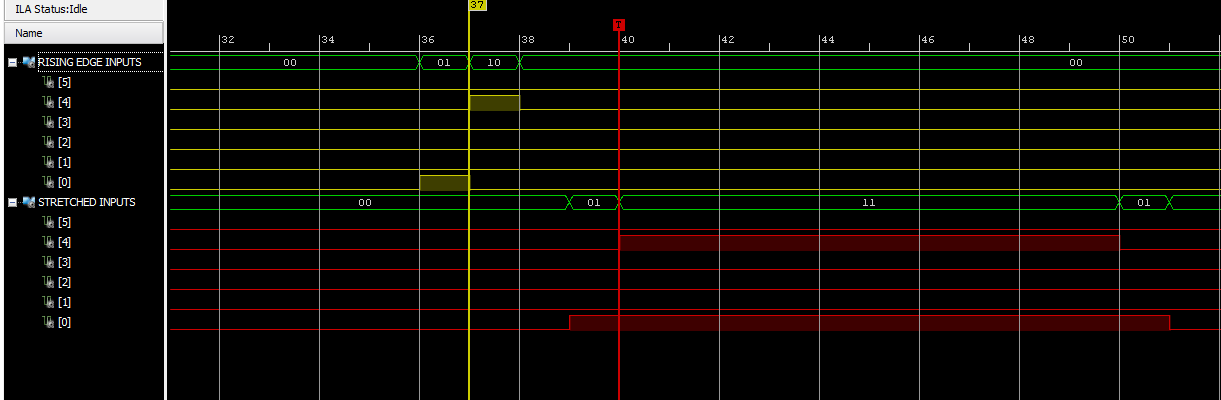
\includegraphics[width=.90\textwidth]{./Images/Initial.png}
  \caption{Input pulses (yellow) and corresponding stretched signals (red). Input 0 is stretched by 10 cycles, input 4 by 8, hence the difference in pulse widths.}
  \label{Fig:exampleExtendedTriggers}
\end{figure}\\
We can now define the trigger logic to be used to assert a valid trigger: we only consider the lower 32-bits of the trigger word and see how different values can produce very different results.
\begin{itemize}
    \item Trigger \gls{lsb} word= 0x00020000. This indicates that the only valid trigger combination occurs when both \emph{in0} and \emph{in4} are high. The valid trigger goes high 1 clock cycle after this condition is met and remains high up to 1 clock cycle after the condition is no longer valid. This is illustrated in figure~\ref{Fig:exampleTrig00020000}.
        \begin{figure}
            \centering
            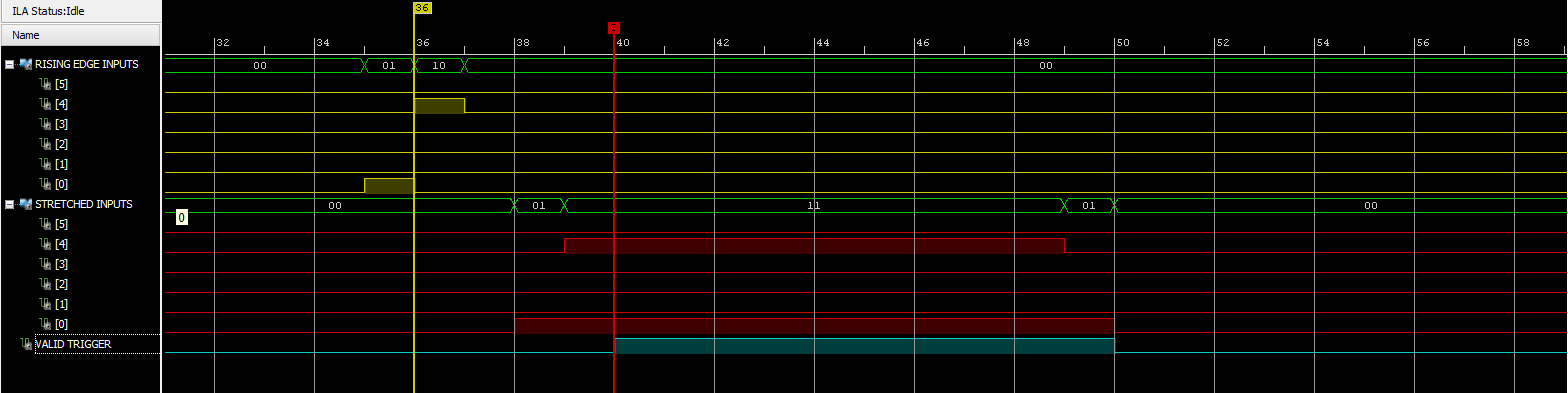
\includegraphics[width=.90\textwidth]{./Images/Trigger0x00020000.png}
            \caption{Trigger configuration 0x00020000. The valid trigger (blue) is asserted only when both signals are high. This condition occurs at frame 39. The trigger is asserted on the following frame.}
            \label{Fig:exampleTrig00020000}
        \end{figure}\\
    \item Trigger \gls{lsb} word= 0x00020002. This indicates that a valid trigger is achieved in two separated configurations (in logic OR): when both inputs are high at the same time (as in the previous case) or if \emph{in0} is active on its own. This is illustrated in figure~\ref{Fig:exampleTrig00020002}. It can be seen that the valid trigger is asserted immediately one clock cycle after \emph{in0} is high and remains high as long as this condition is met. One might assume that specifying the combination with input 4 is redundant, but the following example should show that this is not the case.
        \begin{figure}
            \centering
            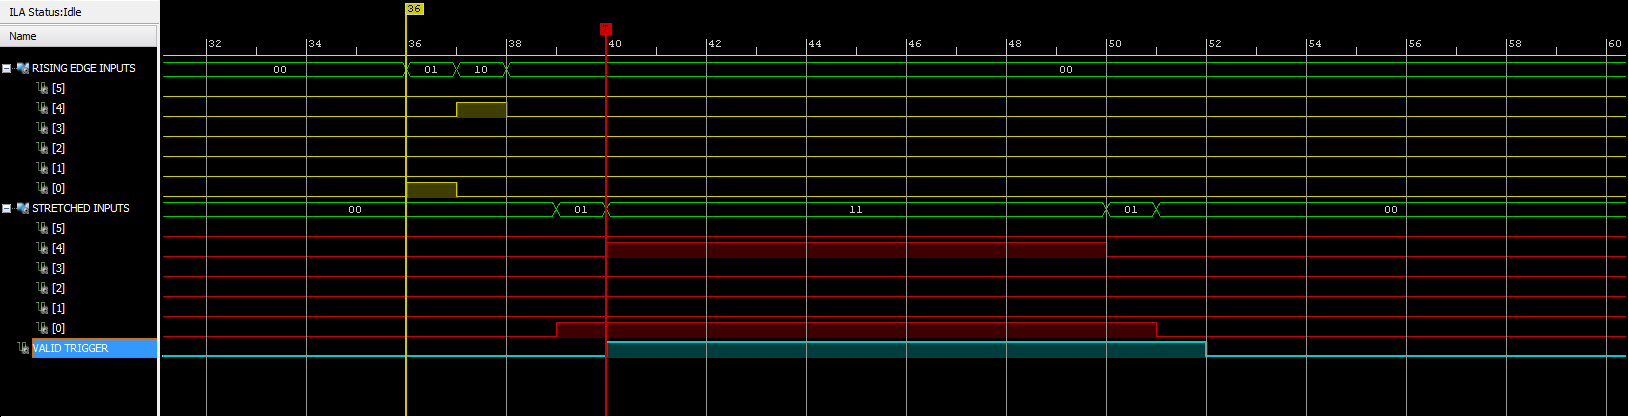
\includegraphics[width=.90\textwidth]{./Images/Trigger0x00020002.png}
            \caption{Trigger configuration 0x00020002. The valid trigger (blue) is asserted if \emph{in0} is high OR when \emph{in0} and \emph{in4} are both high at the same time.}
            \label{Fig:exampleTrig00020002}
        \end{figure}\\
    \item Trigger \gls{lsb} word= 0x00000002. This indicates that the only valid configuration is the one where only \emph{in0} is high. It is important to understand that in this configuration all other inputs act as veto. This might produce unexpected results if the user is not careful\footnote{Specifically, pulse stretch, pulse delay and trigger logic must be configured correctly to avoid unwanted results.}.\\
        In figure~\ref{Fig:exampleTrig00000002} it is possible to see that the logic produces two separated trigger valid pulses, both shorter than the ones in previous examples: the first one is due to \emph{in0} going high while \emph{in4} is low. As soon as \emph{in4} goes high, the trigger condition is no longer met. When \emph{in4} returns low, a trigger condition is met again because \emph{in0} is still high. In this specific case, the double pulse is caused by the different width of the pulses.
        \begin{figure}
            \centering
            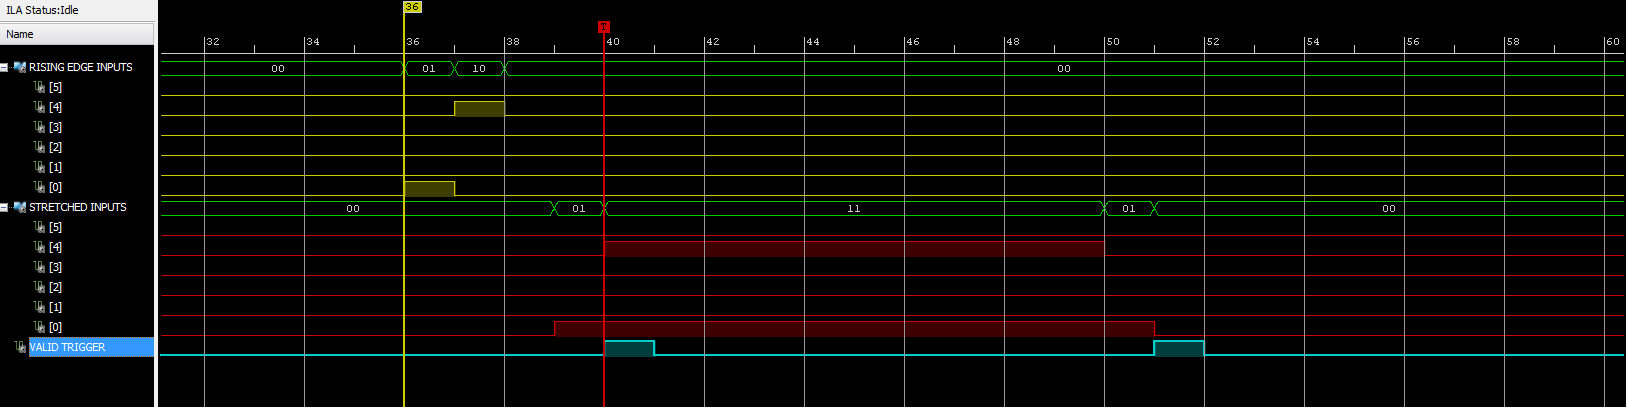
\includegraphics[width=.90\textwidth]{./Images/Trigger0x00000002.png}
            \caption{Trigger configuration 0x00000002. The valid trigger (blue) is asserted only when \emph{in0} is active on its own. As such, two separated trigger pulses are produced because \emph{in4} goes high and returns low before \emph{in0}.}
            \label{Fig:exampleTrig00000002}
        \end{figure}\\
\end{itemize}
